\chapter{Linear Methods for Classification} \label{chapLinearClassification}

%citazione introduttiva
\epigraph{\textit{People label people; algorithms too.}}{}

Differently from regression models, classification models aim at predicting a categorical target variable $k\in K$.\footnote{The package logproj provides methods to deal with linear classification \href{https://github.com/aletuf93/logproj/blob/master/logproj/M_learningMethod/linear_models.py}{here}.}  The input space where the predictors $X$ lies can always be divided into a set of regions divided by decision boundaries according to the values of $G$. A statistical model with a discrete target variables aims at describing a function $F$ as:

\begin{equation}
\Pr{(G=k)}=F(x^T\beta)
\label{eq_classification1}
\end{equation}

Where $G$ is a discrete value assuming values $k\in K$ and $F$ is a function of an input vector $x$ and a vector of unknown parameters $\beta$. In general, the OLS model is not a good model since its domain is continuous. In this case, it is necessary to provide a different probability model with the following characteristics:

\begin{equation}
f(X)=\left\{
                \begin{array}{ll}
                  \lim_{x^T\beta \to -\infty} F\left(x^T\beta\right)=0 \\
                  \lim_{x^T\beta \to +\infty} F\left(x^T\beta\right)=1 \\
                \end{array}
              \right.
\label{eq_classification2}
\end{equation}

A cumulative distribution function (CDF) has both these features and it is chosen as a model, for this reason. Two very common CDF functions are used.

\begin{enumerate}
    \item Probit (probability unit) function (CDF of the gaussian distribution function)
    \begin{equation}
        \Pr{\left(G=1\right)}=F_p\left(x^T\beta\right)=\int_{-\infty}^{x^T\beta/\sigma}{\frac{1}{2\pi}e^{-\frac{z^2}{2}}dz}
        \label{eq_probit}
    \end{equation}
    
    \item Logit (logistic unit) function (CDF of the logistic distribution function)
    \begin{equation}
        \Pr{\left(G=1\right)}=F_l\left(x^T\beta\right)=\int_{-\infty}^{x^T\beta/\sigma}{\frac{e^z}{\left(1+e^z\right)^2}dz}=\frac{e^{x^T\beta}}{1+e^{x^T\beta}}
        \label{eq_logit}
    \end{equation}
    
\end{enumerate}

In particular, the logit function can be linearized to build a linear classification model (see section \ref{secLogisticRegression}). To compare two classes (i.e., to define a boundary between them) the odds ratio $\frac{p}{1-p}$ are considered. A decision boundary is defined where an odd ratio is equal to zero. In general, the $\Pr{\left(G=k\middle| X=x\right)}$ is defined according to different statistical distributions. Let assume:

\begin{itemize}
    \item $f_{k\left(x\right)}$ is the class density of $X$ in class $G=k$;
    \item $\pi_k$ is the prior probability of class $k$ (with $\sum_{k=1}^{K}{\pi_k=1}$).
\end{itemize}

By applying the Bayes theorem (see equation (\ref{eq_bayesTheorem})), we have:

\begin{equation}
        \Pr{\left(G=k\middle| X=x\right)}=\frac{f_k\left(x\right)\pi_k}{\sum_{l=1}^{K}{f_l\left(x\right)\pi_l}}
        \label{eq_classificationModels}
\end{equation}

Each classification model assumes or uses a different way to define $f_{k\left(x\right)}$. When it exists a monotone transformation of $\Pr(G=k|X=x)$ which make it linear in $X$, then the prediction model is linear. All these models use the $\Pr{\left(G=k\middle| X=x\right)}$ to define discriminant functions $\delta_k(x)$ such that an entry $x$ is classified by the model into one of the $k$ class maximising $\delta_k(x)$.\par

In general, classification aims at dividing the hyperplanes into a number of subspaces equal to the classes of the target variable. This can be done by minimising the distance of misclassified points to the decision boundaries. A simple algorithm explaining this logic is Rosenblatt’s Perceptron Algorithm. A perceptron is a classifier which computes a linear combination of the input feature and returns the sign. If $y_i=-1$, then the point $i$ is misclassified, otherwise $y_i=1$. The objective function of the algorithm is to minimise:

\begin{equation}
        \min{(D\left(\beta,\beta_0\right))}=-\sum_{i\in M}{y_i(x_i^T\beta+\beta_0)}
        \label{eq_perceptron1}
\end{equation}

Where $M$ is the set of misclassified points. The gradient of this function is:

\begin{equation}
        \frac{\partial D\left(\beta,\beta_0\right)}{\partial\beta}=-\sum_{i\in M}{y_ix_i}
        \label{eq_perceptron2}
\end{equation}

\begin{equation}
        \frac{\partial D\left(\beta,\beta_0\right)}{\partial\beta_0}=-\sum_{i\in M} y_i
        \label{eq_perceptron3}
\end{equation}

The algorithm visits in a sequence all the misclassified points and updates the parameter $\beta$.

\begin{equation}
        \left(\begin{matrix}\beta\\\beta_0\\\end{matrix}\right)\gets\left(\begin{matrix}\beta\\\beta_0\\\end{matrix}\right)+\rho\left(\begin{matrix}y_ix_i\\y_i\\\end{matrix}\right)
        \label{eq_perceptron4}
\end{equation}

$\rho$ is called “learning rate”, and it can be proved that this algorithm converges when the classes are linearly separable.

\section{Model selection}
Similarly to the error metrics evaluating regression models, classification models have specific error metrics to compare the outcome of each model and choose the one with the best predictive performance.

\subsection{Accuracy}
The accuracy is the simplest indicator since it measures the number of good predictions over the total number of predictions. We consider the case of binary classification (i.e., two classes '1', and '-1') and the number of the:

\begin{itemize}
    \item true positives $TP$: the items with true label '1', classified correctly;
    \item true negatives $TN$, the items with true label '-1', classified correctly;
    \item false positives $FP$, the items with true label '-1', classified incorrectly;
    \item false negatives $FN$, the items with true label '1', classified incorrectly.
\end{itemize}
Accuracy is calculated as follows:

\begin{equation}
        Accuracy=\frac{TN+TP}{TN+TP+FN+FP}
        \label{eq_accuracy}
\end{equation}

Accuracy can also be defined for every single class (per-class accuracy) to avoid class skewness (i.e. an imbalanced number of samples among classes in the training dataset).

\subsection{Confusion matrix}
A confusion matrix (see Figure \ref{fig_confusionMatrix}) is a visualization tool used to identify the number of correctly or incorrectly classified points. A confusion matrix is useful when the error generated by a false positive and the one generated by a false negative have different relevance in practice which accuracy is not able to detect (since it averages all positives and negatives together).

% INSERT fig_confusionMatrix
\begin{figure}[hbt!]
\centering
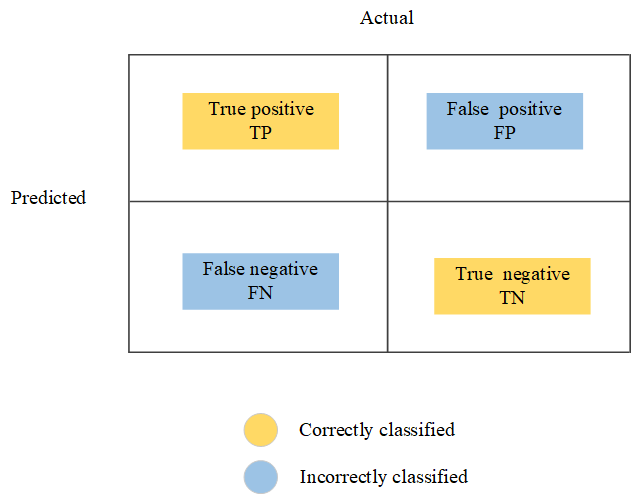
\includegraphics[width=1\textwidth]{SectionLetsMath/linearClassification_figures/fig_confusionMatrix.png}
\captionsetup{type=figure}
\caption{Example of a confusion matrix.}
\label{fig_confusionMatrix}
\end{figure}

\subsection{Log-loss}
Log-loss can be used as a “soft” (see section \ref{secClustering}) measure of accuracy when the classifier outputs a probability that an observation belongs to a class (or another). Log-loss is calculated as:

\begin{equation}
    log-loss=-\frac{1}{N}\sum_{i=1}^{N}{y_i\log{(p_i)}+(1-y_i)\log(1-p_i)}
    \label{eq_logloss}
\end{equation}
This definition of log-loss is similar to the cross-entropy in the information theory, which measures the unpredictability of something. In practice, by minimising the cross-entropy, the accuracy is maximised.

\subsection{AUC}
The area under the curve (AUC) is a scalar indicator calculated as the area of a Receiver Operating Characteristic (ROC) curve. The ROC curve shows the sensitivity of the classifier by plotting the rate of true positives to the rate of false positives. The sensitivity of a classifier is defined as follows.

\begin{equation}
    True\ positive\ rate\ =\ specificity=\frac{TN}{FP+TN}
    \label{eq_specificity}
\end{equation}

\begin{equation}
    False\ positive\ rate=1-specificity=\frac{FP}{FP+TN}
    \label{eq_falsePositiveRate}
\end{equation}

Specificity, together with specificity, is used to define the ROC curve. A ROC curve defines the performance of a classifier by plotting the false positive rate on the x-axis, and the true positive rate on the y-axis. An ideal classifier (classifying observations 100\% correctly) would go to a 100\% rate of true positives immediately. This is unlike to happen in practice, but the faster the curve to go closer to 100\%, the better the classifier. To quickly compare the performance of different models, the area under the ROC curve is calculated, and the higher the area, the better the performance of the classifier.

\subsection{Precision and recall}
Based on the confusion matrix, it is possible to identify other metrics to evaluate the classification model. There is no optimal evaluation metric. The choice of the metric depends on the problem instance and the risk of misclassification into false positives or false negatives.

\begin{equation}
    Precision=\frac{TP}{TP+FP}
    \label{eq_precision}
\end{equation}

\begin{equation}
    Recall=Sensitivity=\frac{TP}{TP+FN}
    \label{eq_recall}
\end{equation}

Precision gives importance to the cost of false-positive. It answers the question \textit{“Out of the items that the classifier predicted to be relevant, how many are truly relevant?”} On the other side, sensitivity (or recall) gives importance to the cost of a false negative. Answering the question: \textit{“Out of all the items that are truly relevant, how many are detected by the classifier?”}. Precision and recall can be matched together by plotting a precision versus recall curve (similar to a ROC curve) or calculating the so-called F1 score.

\begin{equation}
    F1=\frac{2\times precision\times recall}{precision+recall}
    \label{eq_f1Score}
\end{equation}
A low F1 score indicates that either precision or recall is small.

\section{Linear Discriminant Analysis}
Linear Discriminant Analysis (LDA) assumes the decision boundaries being linear. In particular, each class $k$ is assumed having Gaussian density (defined by a multivariate Gaussian distribution), consequently:

\begin{equation}
    f_k\left(x\right)=\frac{1}{\left(2\pi\right)^\frac{p}{2}\left|\Sigma_k\right|^\frac{1}{2}}e^{-\ \frac{1}{2}\left(x-\mu_k\right)^T\Sigma_k^{-1}(x-\mu_k)}
    \label{eq_LDA1}
\end{equation}

LDA assumes all classes $k$ has the same covariance matrix $\Sigma$. Under this hypothesis, the equation describing the decision boundaries remains a linear function of $x$.To compare two classes $k$ and $l$ defining decision boundaries, the log ratio is considered.

\begin{equation}
    \begin{split}
        \log{\left(\frac{Pr{\left(G=k\middle| X=x\right)}}{Pr{\left(G=l\middle| X=x\right)}}\right)}= \log{\left(\frac{f_k\left(x\right)}{f_l\left(x\right)}\right)}+\log{\left(\frac{\pi_k}{\pi_l}\right)}= \\    
        = \log{\left(\frac{\pi_k}{\pi_l}\right)}-\frac{1}{2}\left(\mu_k+\mu_l\right)^T\Sigma^{-1}\left(\mu_k-\mu_l\right)+x^T\Sigma^{-1}(\mu_k-\mu_l)\\
    \end{split}
    \label{eq_LDA2}
\end{equation}

Decision boundaries are found where the equation (\ref{eq_LDA2}) equals zero. Assuming that all classes have an equal covariance matrix $\Sigma_k=\Sigma\ \forall k$ implies that the decision boundaries are linear in $x$. In other words, the $p$-dimensional space $\mathbb{R}^p$, where the points in $X$ lie, is divided by hyperplanes (for example, when $X\in \mathbb{R}^2$ i.e., $p=2$ the plane is divided by a number of straight lines). The resulting discriminant function is as follows.

\begin{equation}
    \delta_k\left(x\right)=x^T\Sigma^{-1}\mu_K-\frac{1}{2}\mu_k^T\Sigma^{-1}\mu_k+\log{\pi_k}
    \label{eq_LDA3}
\end{equation}

In practice, the model assumes a certain distribution of the data (the multivariate Gaussian) estimating the parameters as follows. Given the number $N_k$ of the observations for each class $k$, having

\begin{equation}
    {\hat{\pi}}_k=\frac{N_k}{N}
    \label{eq_LDA4}
\end{equation}

\begin{equation}
    {\hat{\mu}}_k=\sum_{g_i=k}\frac{x_i}{N_k}
    \label{eq_LDA5}
\end{equation}

\begin{equation}
    \hat{\Sigma}=\sum_{k=1}^{K}\sum_{g_i=k}\frac{\left(x_i-{\hat{\mu}}_k\right)\left(x_i-{\hat{\mu}}_k\right)^T}{N-K}
    \label{eq_LDA6}
\end{equation}

In general, when the covariance matrix $\Sigma_k$ are different, the discriminant functions are quadratic (QDA).

\begin{equation}
    \delta_k\left(x\right)=-\frac{1}{2}\log{\left|\Sigma_k\right|-\frac{1}{2}}\left(x-\mu_k\right)^T\Sigma_k^{-1}\left(x-\mu_k\right)+\log{\pi_k}
    \label{eq_LDA7}
\end{equation}

It is possible to apply LDA as well, by shrinking the covariance matrices, using an hyperparameter $\alpha$ and then applying LDA.

\begin{equation}
    \hat{\Sigma}\left(\alpha\right)=\alpha{\hat{\Sigma}}_k+\left(1-\alpha\right)\hat{\Sigma}
    \label{eq_LDA8}
\end{equation}


\section{Logistic Regression} \label{secLogisticRegression}

Similarly to LDA, Logistic regression is a linear model used to predict the value of a discrete variable. The model has the form:

\begin{equation}
\begin{split}
    \log{\left(\frac{\Pr{\left(G=1\middle| X=x\right)}}{\Pr{\left(G=K\middle| X=x\right)}}\right)=\beta_{10}+\beta_1^Tx} \\
    \log{\left(\frac{\Pr{\left(G=2\middle| X=x\right)}}{\Pr{\left(G=K\middle| X=x\right)}}\right)=\beta_{20}+\beta_2^Tx} \\
    \ldots \\
    \log{\left(\frac{\Pr{\left(G=K-1\middle| X=x\right)}}{\Pr{\left(G=K\middle| X=x\right)}}\right)=\beta_{(K-1)0}+\beta_{(K-1)}^Tx} \\
\end{split}
\label{eq_LogisticRegression1}
\end{equation}

The model uses $K-1$ classes while the $K$-th class can be arbitrarily chosen and is always found in the denominator of the model. Differently from LDA (where linearity is given by the assumption of Gaussian parameter), logistics regression does not assume the distribution of $X$, but it is linear by construction. To get a simplified notation we introduce $\theta={\beta_{10},\ldots{,\beta}_{\left(K-1\right)0};\beta_1^T,\ldots,\beta_{K-1}^T}$, and

\begin{equation}
    \Pr{\left(G=k\middle| X=x\right)}=p_k(x,\theta)
    \label{eq_LogisticRegression2}
\end{equation}

Since the probability distribution of $x$ is not given apriori, it is not possible to develop the equation and get a closed-form formula to fit the model. A maximum likelihood estimator (MLE) is, then, used to fit the model and get $\beta$. A multinomial distribution is appropriate to define the distribution of $\Pr{\left(G\middle| X\right).\ }$ Here the case of  $K=2$ is discussed for brevity. Using the multinomial distribution, the formula of the log-likelihood\footnote{Log-likelihood is used since the logarithm is an increasing function and it is equivalent to maximize the likelihood or the log-likelihood. In this application and many other cases, maximizing a logarithm results much more simple.} of $\beta$ is:

\begin{equation}
    l\left(\beta\right)=\sum_{i=1}^{N}{{y_i\log{\left(p\left(x_i;\beta\right)\right)}+\left(1-y_i\right)\log{\left(1-p\left(x_i;\beta\right)\right)}}}
    \label{eq_LogisticRegression3}
\end{equation}

To get an MLE the $\frac{\partial l\left(\beta\right)}{\partial\beta}$ is computed, set to zero and solved in $\beta$. This implies solving $p+1$ non-linear equations in $\beta$. The calculus can be done using the Newton-Raphson algorithm which usually converges since log-likelihood is concave.

\section*{Further reading}
Supplementary reading materials can be found in \cite{Bramer2016}.

%\clearpage
\bibliographystyle{ieeetr}
\bibliography{SectionLetsMath/linearclassification_ref}